% Modelo UFSC/CTC/DAS para PFCs (08/07/2020)
% Autores: Matheus Bruhns Bastos e Marcelo De Lellis Costa de Oliveira
% --------------------------------------------------------
% Adaptado do arquivo Template-Trabalhos-Academicos-UFSC-A4-v1.3
% disponibilizado em http://portal.bu.ufsc.br/files/2013/10/Template-Trabalhos-Academicos-UFSC-A4-v1.3.zip
% Modelo UFSC para Trabalhos Academicos (tese de doutorado, dissertação de
% mestrado) utilizando a classe abntex2
%
% Autor: Alisson Lopes Furlani
% 	Modificações:
%	- 27/08/2019: Alisson L. Furlani, add 'glossaries' package
%   - 30/10/2019: Alisson L. Furlani, adjusted some spacing errors and changed math fonts
%   - 17/01/2020: Alisson L. Furlani, updated certification page
%   - 07/02/2020: Alisson L. Furlani, fixed table counter bug
%   - 11/03/2020: Alisson L. Furlani, changed greek letters in math and fixed citation style
% ------------------------------------------------------------------------
% ------------------------------------------------------------------------

\documentclass[
	% -- opções da classe memoir --
	12pt,				% tamanho da fonte
	%openright,			% capítulos começam em pág ímpar (insere página vazia caso preciso)
	oneside,			% para impressão no anverso. Oposto a twoside
	a4paper,			% tamanho do papel. 
	% -- opções da classe abntex2 --
	chapter=TITLE,		% títulos de capítulos convertidos em letras maiúsculas
	section=TITLE,		% títulos de seções convertidos em letras maiúsculas
	%subsection=TITLE,	% títulos de subseções convertidos em letras maiúsculas
	%subsubsection=TITLE,% títulos de subsubseções convertidos em letras maiúsculas
	% -- opções do pacote babel --
	brazil,			% idioma adicional para hifenização
	%french,				% idioma adicional para hifenização
	%spanish,			% idioma adicional para hifenização
	english				% o último idioma é o principal do documento
	]{abntex2}

\usepackage{setup/ufscthesisA4-alf}
\addbibresource{aftertext/bibliografia.bib} % Seus arquivos de referências
% \usepackage{hyperref}
\usepackage{amsmath,amssymb}    % Para os simbolos de lógica temporal
% \usepackage{stix2}              % Para simbolos de LT mais específicos ainda
\usepackage{pict2e}
\usepackage{accsupp}
\usepackage{tikz}
\usepackage{stackengine, graphicx} %
\usepackage{tikz}
\usetikzlibrary{automata, positioning, arrows.meta}
% \graphicspath{{Latex - English/}}

% ---
% Filtering and Mapping Bibliographies
% ---
\DeclareSourcemap{
	\maps[datatype=bibtex]{
		% remove fields that are always useless
		\map{
			\step[fieldset=abstract, null]
			\step[fieldset=pagetotal, null]
		}
		% remove URLs for types that are primarily printed
%		\map{
%			\pernottype{software}
%			\pernottype{online}
%			\pernottype{report}
%			\pernottype{techreport}
%			\pernottype{standard}
%			\pernottype{manual}
%			\pernottype{misc}
%			\step[fieldset=url, null]
%			\step[fieldset=urldate, null]
%		}
		\map{
			\pertype{inproceedings}
			% remove mostly redundant conference information
			\step[fieldset=venue, null]
			\step[fieldset=eventdate, null]
			\step[fieldset=eventtitle, null]
			% do not show ISBN for proceedings
			\step[fieldset=isbn, null]
			% Citavi bug
			\step[fieldset=volume, null]
		}
	}
}
% ---

% ---
% Informações de dados para CAPA e FOLHA DE ROSTO
% ---
% FIXME Substituir 'Nome completo do autor' pelo seu nome.
\autor{Rafael Ramildes Ferreira}
% FIXME Substituir 'Título do trabalho' pelo título da trabalho.
\titulo{Runtime verification in low level software in the ProVANT project}
% FIXME Substituir 'Subtítulo (se houver)' pelo subtítulo da trabalho.  
% Caso não tenha substítulo, comente a linha a seguir.
% \subtitulo{Subtitle (if any)}
% FIXME Substituir 'XXXXXX' pelo nome do seu
% orientador.
\orientador{Prof. Leandro Buss Becker, Dr.}
% FIXME Se for orientado por uma mulher, comente a linha acima e descomente a linha a seguir.
% \orientador[Orientadora]{Nome da orientadora, Dra.}
% FIXME Substituir 'XXXXXX' pelo nome do seu
% supervisor no local de realização do PFC. Caso não tenha supervisor, comente a linha a seguir.
% \coorientador{XXXXXX, Eng.}
% FIXME Se for supervisionado por uma mulher, comente a linha acima e descomente a linha a seguir.
% \coorientador[Supervisora]{XXXXXX, Eng.}
% FIXME Substituir '[ano]' pelo ano (ano) em que seu trabalho foi defendido.
\ano{2024}
% FIXME Substituir '[dia] de [mês] de [ano]' pela data em que ocorreu sua defesa.
%\data{[dia] de [mês] de [ano]}
% FIXME Substituir 'Local' pela cidade em que ocorreu sua defesa.
\local{Florianópolis}
\instituicaosigla{UFSC}
\instituicao{Federal University of Santa Catarina}
% FIXME Substituir 'Dissertação/Tese' pelo tipo de trabalho (Tese, Dissertação). 
\tipotrabalho{Final report of the subject DAS5511 (Course Final Project) as a Concluding Dissertation}
%Relatório final da disciplina DAS5511 (Projeto de Fim de Curso) como Trabalho de Conclusão}
\formacao{Control and Automation Engineer}
% FIXME Substituir '[mestrado/doutorado]' pelo nivel adequado.
% \nivel{[mestrado/doutorado]}
% FIXME Substituir 'Programa de Pós-Graduação em XXXXXX' pela curso adequado.
% \programa{Programa de Pós-Graduação em XXXXXX}
\centro{Technology Center}
\departamento{Automation and Systems Engineering Department}
\curso{Undergraduate Course in Control and Automation Engineering}
\preambulo
{%
%\imprimirtipotrabalho~do~\imprimircurso~da~\imprimirinstituicao~como~requisito~para~a~obtenção~do~título~de~\imprimirformacao.
\imprimirtipotrabalho~of the~\imprimircurso~of the~\imprimirinstituicao.
}
% ---

% ---
% Configurações de aparência do PDF final
% ---
% alterando o aspecto da cor azul
\definecolor{blue}{RGB}{41,5,195}
% informações do PDF
\makeatletter
\hypersetup{
     	%pagebackref=true,
		pdftitle={\@title}, 
		pdfauthor={\@author},
    	pdfsubject={\imprimirpreambulo},
	    pdfcreator={LaTeX with abnTeX2},
		pdfkeywords={ufsc, latex, abntex2}, 
		colorlinks=true,       		% false: boxed links; true: colored links
    	linkcolor=black,%blue,          	% color of internal links
    	citecolor=black,%blue,        		% color of links to bibliography
    	filecolor=black,%magenta,      		% color of file links
		urlcolor=black,%blue,
		bookmarksdepth=4
}
\makeatother
% ---

% ---
% compila a lista de abreviaturas e siglas e a lista de símbolos
% ---

% Declaração das siglas
\siglalista{ABNT}{Associação Brasileira de Normas Técnicas}
\siglalista{RV}{Runtime Verification}
\siglalista{SCS}{Safety-Critical Systems}
\siglalista{CPS}{Cyber-Physical Systems}
\siglalista{RM}{Runtime Monitoring}
\siglalista{FPGA}{Field Programmable Gate Array}
\siglalista{TL}{Temporal Logic}
\siglalista{UML}{Unified Modeling Language}
\siglalista{AADL}{Architecture Analysis \& Design Language}
\siglalista{LLH}{Low Level Hardware}
\siglalista{HLH}{High Level Hardware}
\siglalista{GPU}{Graphics Processing Unit}
\siglalista{IMU}{Inertial measurement unit}
\siglalista{GPS}{Global Positioning System}
\siglalista{PWM}{Pulse Width Modulation}
\siglalista{UDP}{User Datagram Protocol}
\siglalista{TCP}{Transmission Control Protocol}
\siglalista{CSMA/CD}{Carrier Sense Multiple Access with Collision Detection}
\siglalista{UAV}{Unmanned Aerial Vehicle}

% Declaração dos simbolos
\simbololista{C}{\ensuremath{C}}{Circunferência de um círculo}
\simbololista{pi}{\ensuremath{\pi}}{Número pi} 
\simbololista{r}{\ensuremath{r}}{Raio de um círculo}
\simbololista{A}{\ensuremath{A}}{Área de um círculo}


% ---
% Simbolos de Lógica Temporal
% ---
\renewcommand{\diamond}{\mdlgwhtdiamond}
\newcommand{\diamonddiamond}{\stackinset{c}{0mm}{c}{0.25mm}{$ \diamond $}{\smwhtdiamond}$}


% compila a lista de abreviaturas e siglas e a lista de símbolos
\makenoidxglossaries 

% ---

% ---
% compila o indice
% ---
\makeindex
% ---

% ----
% Início do documento
% ----
\begin{document}

% Seleciona o idioma do documento (conforme pacotes do babel)
\selectlanguage{english}

% Retira espaço extra obsoleto entre as frases.
\frenchspacing 

% Espaçamento 1.5 entre linhas
\OnehalfSpacing

% Corrige justificação
%\sloppy

% ----------------------------------------------------------
% ELEMENTOS PRÉ-TEXTUAIS
% ----------------------------------------------------------
% \pretextual %a macro \pretextual é acionado automaticamente no início de \begin{document}
% ---
% Capa, folha de rosto, ficha bibliografica, errata, folha de apróvação
% Dedicatória, agradecimentos, epígrafe, resumos, listas
% ---
% ---
% Capa
% ---
\imprimircapa
% ---

% ---
% Folha de rosto
% (o * indica que haverá a ficha bibliográfica)
% ---
\imprimirfolhaderosto*
% ---

% ---
% Inserir a ficha bibliografica
% ---
% http://ficha.bu.ufsc.br/
\begin{fichacatalografica}
	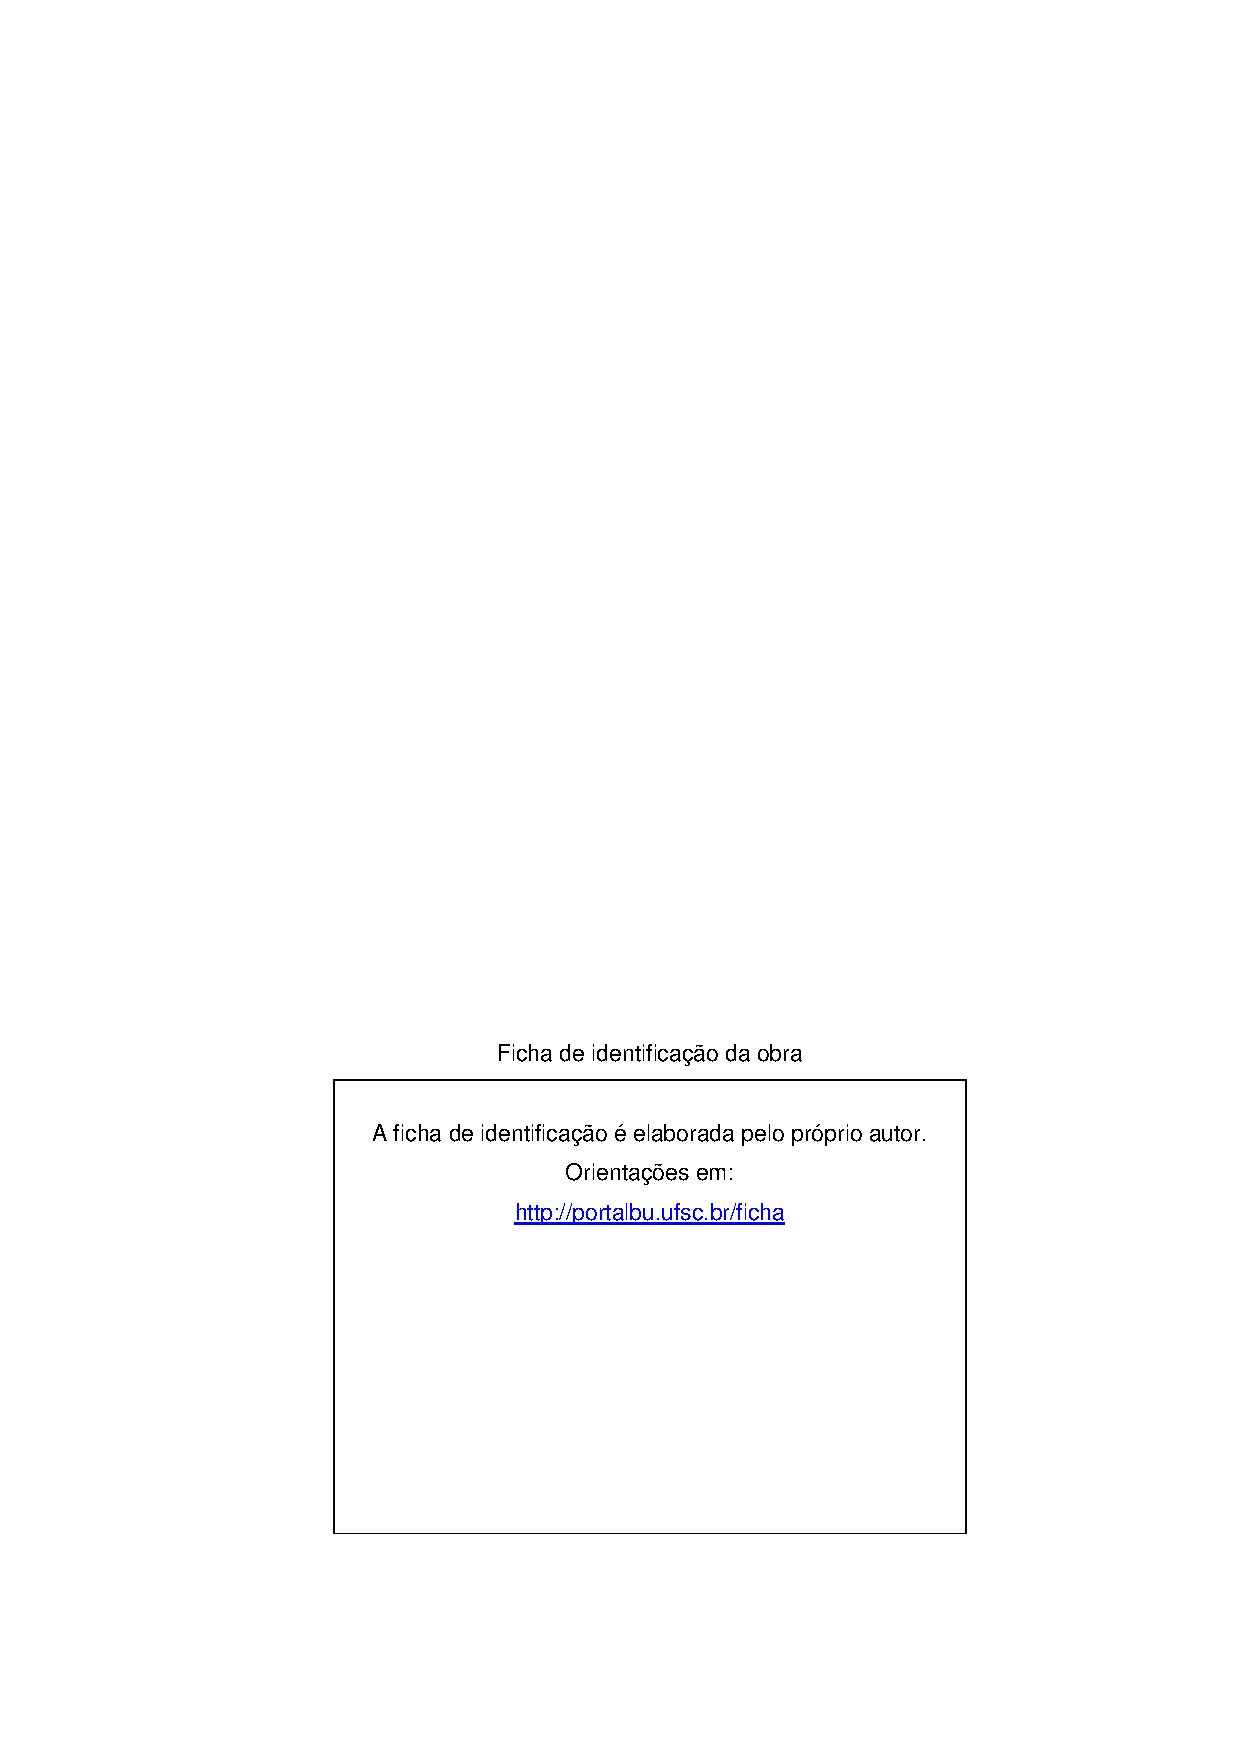
\includepdf{beforetext/Ficha_Catalografica.pdf}
\end{fichacatalografica}
% ---

% ---
% Inserir folha de aprovação
% ---
\begin{folhadeaprovacao}
	\OnehalfSpacing
	\centering
	\imprimirautor\\%
	\vspace*{10pt}		
	\textbf{\imprimirtitulo}%
	\ifnotempty{\imprimirsubtitulo}{:~\imprimirsubtitulo}\\%
	%		\vspace*{31.5pt}%3\baselineskip
	\vspace*{\baselineskip}
	
	This dissertation was evaluated in the context of the subject DAS5511 (Course Final Project) and approved in its final form by the \imprimircurso\\
	%Esta monografia foi julgada no contexto da disciplina DAS5511 (Projeto de Fim de Curso) e aprovada em sua forma final pelo \imprimircurso\\
	\vspace*{\baselineskip}
	Florianópolis, <month> <day>, <year>.\\
	
	%%%%%%%%%%%%%%%%%%%%%%%%%%%%%%%%%%%%%%%%%%%%%
	%IMPORTANT: no signatures are required below!
	%%%%%%%%%%%%%%%%%%%%%%%%%%%%%%%%%%%%%%%%%%%%%
	
	\vspace*{2\baselineskip}
	%\rule{0.4\textwidth}{0.4pt}\\
	Prof. xxxx, Dr.\\
	Course Coordinator\\
	
	\vspace*{\baselineskip}
	\textbf{Examining Board:} \\
	
	
	\vspace*{2\baselineskip}
	%\rule{0.4\textwidth}{0.4pt}\\
	Prof. xxxx, Dr.\\
	Advisor \\
	UFSC/CTC/EAS\\
	
	\vspace*{2\baselineskip}
	%\rule{0.4\textwidth}{0.4pt}\\
	xxxx, Eng.\\
	Supervisor \\
	Company/University xxxx\\
	
	\vspace*{2\baselineskip}
	%\rule{0.4\textwidth}{0.4pt}\\
	Prof. xxxx, Dr.\\
	Evaluator \\
	Institution xxxx\\
	
	\vspace*{2\baselineskip}
	%\rule{0.4\textwidth}{0.4pt}\\
	Prof. xxxx, Dr.\\
	Board President \\
	UFSC/CTC/EAS
\end{folhadeaprovacao}
% ---

% ---
% Dedicatória
% ---
\begin{dedicatoria}
	\vspace*{\fill}
	\noindent
	\begin{adjustwidth*}{}{5.5cm} 
		\raggedleft       
		This work is dedicated to my classmates and my dear parents.
	\end{adjustwidth*}
\end{dedicatoria}
% ---

% ---
% Agradecimentos
% ---
\begin{agradecimentos}
	Inserir os agradecimentos aos colaboradores à execução do trabalho. 
	
	Xxxxxxxxxxxxxxxxxxxxxxxxxxxxxxxxxxxxxxxxxxxxxxxxxxxxxxxxxxxxxxxxxxxxxx. 
\end{agradecimentos}
% ---

% ---
% Epígrafe
% ---
\begin{epigrafe}
	\vspace*{\fill}
	\begin{flushright}
		\textit{``Texto da Epígrafe.\\
			Citação relativa ao tema do trabalho.\\
			É opcional. A epígrafe pode também aparecer\\
			na abertura de cada seção ou capítulo.\\
			Deve ser elaborada de acordo com a NBR 10520.''\\
			(SOBRENOME do autor da epígrafe, ano)}
	\end{flushright}
\end{epigrafe}
% ---

% ---
% DECLARAÇÃO DE PUBLICIDADE
% ---

\begin{center}
	\textbf{DISCLAIMER}
\end{center}

% Atenção: atualize o conteúdo de <texto>.

<City name>, <month> <day>-th, <year>.

\vspace{1cm}

As representative of the <PFC institution of execution> in which the present work was carried out, I declare this document to be exempt from any confidential or sensitive content regarding intellectual property, that may keep it from being published by the Federal University of Santa Catarina (UFSC) to the general public, including its online availability in the Institutional Repository of the University Library (BU). Furthermore, I attest knowledge of the obligation by the author, as a student of UFSC, to deposit this document in the said Institutional Repository, for being it a Final Program Dissertation (\emph{``Trabalho de Conclusão de Curso''}), in accordance with the \emph{Resolução Normativa n° 126/2019/CUn}.

\vspace{15mm}

\begin{center}
	\rule{7cm}{0.7pt} \\
	<Fulano de Tal> \\
	<Instituição de realização do PFC>
\end{center}

\cleardoublepage

% ---
% RESUMOS
% ---

% resumo em português
\setlength{\absparsep}{18pt} % ajusta o espaçamento dos parágrafos do resumo
\begin{resumo}
	\SingleSpacing
	\textbf{Instruções do padrão genérico de TCCs da BU:}
	No Abstract são ressaltados o objetivo da pesquisa, o método utilizado, as discussões e os resultados com destaque apenas para os pontos principais. O Abstract deve ser significativo, composto de uma sequência de frases concisas, afirmativas, e não de uma enumeração de tópicos. Não deve conter citações. Deve usar o verbo na voz ativa e na terceira pessoa do singular. O texto do Abstract deve ser digitado, em um único bloco, sem espaço de parágrafo. O espaçamento entre linhas é simples e o tamanho da fonte é 12. Abaixo do Abstract, informar as palavras-chave (palavras ou expressões significativas retiradas do texto) ou, termos retirados de thesaurus da área. Deve conter de 150 a 500 palavras. O Abstract é elaborado de acordo com a NBR 6028. 
	
	\textbf{Instruções da Coordenação de PFC:} O Abstract deve descrever de forma sucinta: o contexto/motivação/problema tratado no PFC; a solução proposta; a implementação/desenvolvimento; a metodologia e as principais técnicas e ferramentas utilizadas; os principais resultados obtidos e a importância/impactos de tais resultados para a empresa/clientes da empresa/instituto de pesquisa. Escrever todos esses pontos de forma bem resumida e direta, e sem entrar em detalhes técnicos. O tamanho do Abstract deve ocupar praticamente esta página inteira, e num \textbf{único} parágrafo. Além disso, Abstract + Keywords não podem ultrapassar esta página. 
	
	\textbf{Keywords}: Keyword 1. Keyword 2. Keyword 3. \emph{[essas palavras-chave devem obrigatoriamente ser utilizadas no Abstract]}
\end{resumo}

% resumo em inglês
\begin{resumo}[Resumo]
	\SingleSpacing
	\begin{otherlanguage*}{brazil}
		Resumo traduzido para outros idiomas, neste caso, português. Segue o mesmo formato do Abstract.
		
		\textbf{Palavras-chave}: Palavra-chave 1. Palavra-chave 2. Palavra-chave 3.
	\end{otherlanguage*}
\end{resumo}

%% resumo em francês 
%\begin{resumo}[Résumé]
% \begin{otherlanguage*}{french}
%    Il s'agit d'un résumé en français.
% 
%   \textbf{Mots-clés}: latex. abntex. publication de textes.
% \end{otherlanguage*}
%\end{resumo}
%
%% resumo em espanhol
%\begin{resumo}[Resumen]
% \begin{otherlanguage*}{spanish}
%   Este es el resumen en español.
%  
%   \textbf{Palabras clave}: latex. abntex. publicación de textos.
% \end{otherlanguage*}
%\end{resumo}
%% ---

{%hidelinks
	\hypersetup{hidelinks}
	% ---
	% inserir lista de ilustrações
	% ---
	\pdfbookmark[0]{\listfigurename}{lof}
	\listoffigures*
	\cleardoublepage
	% ---
	
	% ---
	% inserir lista de quadros
	% ---
	\pdfbookmark[0]{\listofquadrosname}{loq}
	\listofquadros*
	\cleardoublepage
	% ---
	
	% ---
	% inserir lista de tabelas
	% ---
	\pdfbookmark[0]{\listtablename}{lot}
	\listoftables*
	\cleardoublepage
	% ---
	
	% ---
	% inserir lista de abreviaturas e siglas (devem ser declarados no preambulo)
	% ---
	\imprimirlistadesiglas
	% ---
	
	% ---
	% inserir lista de símbolos (devem ser declarados no preambulo)
	% ---
	\imprimirlistadesimbolos
	% ---
	
	% ---
	% inserir o sumario
	% ---
	\pdfbookmark[0]{\contentsname}{toc}
	\tableofcontents*
	\cleardoublepage
	
}%hidelinks
% ---
% ---

% ----------------------------------------------------------
% ELEMENTOS TEXTUAIS
% ----------------------------------------------------------
\textual

% ---
% 1 - Introdução
% ---
% ----------------------------------------------------------
\chapter{Introduction}
% ----------------------------------------------------------

Over the last 20 year, a plentiful of studies dealt with the \gls{RV} for \gls{SCS}, researching ways of sustaining the desired behavior of \gls{CPS} and a avoiding critical faults.

% \textbf{Instruções do padrão genérico de TCCs da BU:} 

% As orientações aqui apresentadas são baseadas em um conjunto de normas elaboradas pela \gls{ABNT}. Além das normas técnicas, a Biblioteca também elaborou uma série de tutoriais, guias, \textit{templates} os quais estão disponíveis em seu site, no endereço \url{http://portal.bu.ufsc.br/normalizacao/}.

% Paralelamente ao uso deste \textit{template} recomenda-se que seja utilizado o \textbf{Tutorial de Trabalhos Acadêmicos} (disponível neste link \url{https://repositorio.ufsc.br/handle/123456789/180829}).

% Este \textit{template} está configurado apenas para a impressão utilizando o anverso das folhas, caso você queira imprimir usando a frente e o verso, acrescente a opção \textit{openright} e mude de \textit{oneside} para \textit{twoside} nas configurações da classe \textit{abntex2} no início do arquivo principal \textit{main.tex} \cite{abntex2classe}.

% Conforme a \href{https://repositorio.ufsc.br/bitstream/handle/123456789/197121/RN46.2019.pdf?sequence=1&isAllowed=y}{Resolução NORMATIVA nº 46/2019/CPG} as dissertações e teses não serão mais entregues em formato impresso na Biblioteca Universitária. Consulte o Repositório Institucional da UFSC ou sua Secretaria de Pós Graduação sobre os procedimentos para a entrega. 

% \nocite{NBR6023:2002}
% \nocite{NBR6027:2012}
% \nocite{NBR6028:2003}
% \nocite{NBR10520:2002}

% \textbf{Instruções da Coordenação do PFC:} 

% A Introdução deve apresentar um panorama geral do PFC de modo resumido, sem entrar em detalhes técnicos, para que o leitor já entenda aqui na Introdução o começo, meio e fim do PFC. Assim, é muito importante deixar bem claro na Introdução os seguintes pontos (a Introdução pode ser vista como um resumo geral do PFC, e a Seção Resumo como um resumo desse resumo): 

% \begin{itemize}
%      \item O contexto e a motivação do PFC, com uma breve descrição da empresa/instituto de pesquisa (histórico, clientes, produtos, serviços, projetos, etc) em que o PFC foi realizado e do projeto global da empresa em que o PFC está inserido (se for o caso)
%      \item Breve descrição do problema tratado no PFC;
%     \item A importância de tal problema para a empresa/clientes da empresa/instituto de pesquisa;
%     \item Objetivos: aqui são descritos os objetivos, que podem ser estratificados em objetivo geral e objetivos específicos. Outra opção é colocar os objetivos específicos na forma de passos de uma metodologia de trabalho, ou seja, os procedimentos e ferramentas adotadas em cada fase do projeto (um plano de trabalho).
%     \item Breve descrição da solução proposta;
%     \item Breve descrição da implementação/desenvolvimento realizado;
%     \item Breve descrição da metodologia e das principais técnicas e ferramentas utilizadas (do ponto de vista técnico). \textbf{Importante}: como \emph{Scrum} é uma metodologia geral de execução de projetos, ele não se enquadra aqui, pois não se trata de uma metodologia técnica específica para o desenvolvimento do PFC;
%     \item Breve descrição dos principais resultados obtidos e da importância/impactos de tais resultados para a empresa/clientes da empresa/instituto de pesquisa;
%     \item Deixar bem claro o que foi de fato foi realizado pelo(a) autor(a), diferenciando do que foi aproveitado de trabalhos anteriores/outras times da empresa. \textbf{Importante}: esta preocupação em diferenciar o trabalho realizado pelo(a) autor(a) daquele de possíveis colegas de um time deve permear todo o documento.
% \end{itemize}

% Ressaltamos a seguir alguns aspectos cruciais para a escrita do PFC:
% \begin{itemize}
% 	\item Apesar de o tamanho da monografia não ter uma correlação direta com a nota, bons trabalhos costumam ter de 60 a 70 páginas efetivamente escritas (desde a Introdução até a Conclusão, excluindo-se Capa, Resumo, Sumário, Referências Bibliográficas, etc).  Por outro lado, acima de 100 páginas a monografia pode se tornar ``massante'', discorrendo além do necessário para o entendimento do trabalho e, consequentemente, perdendo o foco do leitor.
% 	\item A linguagem a ser utilizada em um trabalho acadêmico deve ser técnico-científica e, portanto, formal (e não informal, como se o trabalho estivesse sendo explicado a um colega ou familiar). Desse modo, não devem ser usadas gírias. Além disso, não se deve escrever ``o trabalho feito por mim'', mas sim algo como ``o presente trabalho trata de/o trabalho realizado pelo(a) autor(a)/etc''.
% 	\item Utilize corretor ortográfico, verifique a gramática, e revise com muito cuidado e atenção todo o texto: pontuação, uso da vírgula, concordância, coesão e clareza textual, encadeamento entre frases, sentenças e parágrafos, etc.
% 	\item Este documento deve corresponder a uma monografia acadêmica, em que se deve fundamentar e justificar as ideias, afirmações, métodos e deduções apresentadas com base em técnicas, ferramentas, metodologias, equações, normas, literatura especializada (livros e artigos), etc, e não a um relatório descritivo voltado a um departamento/time de uma empresa. 
% 	\item As referências bibliográficas não podem conter apenas sites, blogs e manuais técnicos: devem também conter livros, artigos, dissertações, teses, etc. Além disso, há uma diferença entre citação \emph{direta} (comando \verb!\citeas!) e citação \emph{indireta} (comando \verb!\cite!).
% \end{itemize}

% \section*{Estrutura do documento}

% Ao final da Introdução (que é o Capítulo 1), costuma-se apresentar como o documento está organizado, descrevendo brevemente o que é tratado nos demais capítulos do Sumário, começando pelo Capítulo 2. A estrutura de capítulos mostrada no Sumário deste documento é apenas uma sugestão geral e não precisa ser seguida à risca: dependendo da área e do foco do trabalho, tanto a estrutura detalhada (Capítulos, Seções e Subseções) quanto o número de capítulos pode variar. O(A) estudante deve consultar seu(sua) Orientador(a) Acadêmico(a) para definir a estrutura detalhada do documento.

% \noindent\textbf{Exemplo}:

% \emph{O presente documento está organizado da seguinte maneira. O Capítulo~2 apresenta a fundamentação teórica sobre os principais conceitos e técnicas necessárias para o entendimento do problema abordado e da solução proposta. O problema tratado neste PFC é descrito em detalhes no Capítulo~3, juntamente com os requisitos técnicos a serem atendidos. O Capítulo~4 aborda a solução proposta e a metodologia envolvida. O desenvolvimento realizado e a análise dos resultados obtidos são mostrados no Capítulo~5. Por fim, no Capítulo~6, são apresentadas as conclusões deste trabalho e algumas sugestões de trabalhos futuros são elencadas.}


% ---

% ---
% 2 - Capítulo 2
% ---
% ----------------------------------------------------------
\chapter{Technological Background}\label{cap:faults_overall}
% ----------------------------------------------------------

% ----------------------------------------------------------
\section{Runtime Verification}\label{sec:rv}
% ----------------------------------------------------------

\gls{RV} or \gls{RM} is the observance of system behavior during deployment, in order to check or even try to enforce some specification. \cite{falcone_taxonomy_2021,sanchez_survey_2019} It's is normally attempting a formal verification, but restricted to a single trace (the trace that actually got executed in the monitored execution) not being able to verify alternative executions like in Model Checking.

It's normally used in \gls{SCS}, where faults can cause catastrophic consequences. Said systems should be designed with safety in mind, methodically developed by systematical approaches and verified by model checking techniques. The most famous modeling language is the \gls{UML}, but there are other options for embedded system modeling like the \gls{AADL} \cite{feiler_model-based_2013}, which can be used for model checking. However, the model may not be a one to one representation of the system, which can lead to unexpected faults, to avoid and/or detect those \gls{RV} is used.

The system responsible to verify the specification in a \gls{RV} application are generally called monitors. The idea is similar to oracle-based testing, where an observer called oracle is implemented to verify properties of a given test execution. However, as noticed by \textcite{bauer_runtime_2011}, tests typically attempt to be exhaustive, to validate the system during test, while \gls{RV} is only concerned with the current execution. They also count as a difference the fact that \gls{RV} is normally done by synthesize a higher level \gls{TL} language. 

\gls{RV} monitors can be run either online (i.e. together with the application, in real time) or offline (i.e. processing a recorded trace). \cite{bauer_runtime_2011,broering_runtime_2023} For online verification, it's desirable that the monitor be very lightweight so to not interfere with the systems time constraints, or better yet be run in a different processor, core or even in a separate board. In some cases, unobtrusiveness is a required characteristic, for instance to not violate flight certificates, which lead to approaches where the monitor only listens to a existing bus line, being implemented on a dedicated controller or \gls{FPGA}. \cite{rozier_r2u2_nodate}

% ----------------------------------------------------------
\section{Temporal Logic}\label{sec:tl}
% ----------------------------------------------------------

Some authors use the concept of \textit{bad} and \textit{good prefix} as defined by \textcite{kupferman_model_2001}, where a \textit{bad prefix} is a sequence of events that never leads to the fulfillment of the requirements, while the \textit{good prefix} is when any continuation of the trace will be within the specification. % Check this, read the Kupferman article
In \textit{three-valued logic}, as soon as identified by a \gls{RV} monitor, \textit{bad prefix} should return \textit{False}, \textit{good prefix} should return \textit{True}, and any other prefix, yields inconclusive.\cite{bauer_runtime_2011} % I thought he meant it, should be True or False forever, since by the teory, those sequece make so that it can never have a different verdict again, but maybe he doesn't mean that

% But in \gls{RV}, these return values, can not be considered \textit{True} or \textit{False} forever, because, as noted by \textcite{bauer_runtime_2011}, the state observed by a \gls{RV} monitor is define by a set of interest variable, which cannot encapsulate the whole state of the system. So certain caution is to be taken while designing the TV system as unobserved changes in the environment may alter the observed variables % Tá muito ruim isso aqui 

% \textcite{reinbacher_temporal-logic_2014} defines a variation of the \gls{TL} operands $\square_J$ (Globally within the period $J$) and $\diamond_J$ (In the future within the period $J$) represented by $\squareleftblack_\tau$ (Invariant within the next $\tau$ time units) and $\diamondleftblack_\tau$ (that the expression will hold in the next $\tau$ time units). These operands are used in their software, R2U2 \cite{noauthor_r2u2_nodate-1}, simply as G and F 
% (so means the classic definition is not supported) 
and, because of these definition, it is continuously verified, which wouldn't need to be if it used the classic definition, but would be less expressive. % Find a source for the "classic definition" (maybe something in MTL) and think about this text


% \DeclareRobustCommand{\wdcbsd}{%
%   \begingroup
%   \setlength{\unitlength}{\fontcharht\font`T}%
%   \begin{picture}(1,1)
%   \polygon(.5,0)(1,.5)(.5,1)(0,.5)
%   \polygon*(.5,0.2)(.8,.5)(.5,.8)(.2,.5)
%   \end{picture}%
%   \endgroup
% }
% \DeclareUnicodeCharacter{25C8}{\wdcbsd}
\DeclareRobustCommand*{\wdcbsd}{%
  \leavevmode
  \begingroup
    \BeginAccSupp{
      method=hex,
      unicode,
      ActualText=25C8,
      space,
    }%
      \setlength{\unitlength}{\fontcharht\font`\H}%
      \pgfmathsetlength{\unitlength}{cos(45)*\unitlength}%
      \tikz[
        rotate=45,
        x=\unitlength,
        y=\unitlength,
        even odd rule,
      ]\fill
        (0, 0) rectangle (1, 1)
        ++(-.4pt, -.4pt) rectangle (.4pt, .4pt)
        (.25, .25) rectangle (.75, .75)
      ;%
    \EndAccSupp{}%
  \endgroup
}

Similar past-time operands variations are defined by \cite{reinbacher_runtime_2014}, called %\wdcbsd%
% $\diamonddiamond$ $\boxbox$
%\unichar{"25C8}

% \textbf{Instruções da Coordenação do PFC:}

% Deve-se colocar um parágrafo introdutório no início de \textbf{cada} capítulo, descrevendo os assuntos que serão abordados e a relação com o restante do trabalho. Por exemplo: \emph{A Seção 2.1 apresenta \ldots. Os resultados obtidos são analisados na Seção 2.2.} Pode-se fazer o mesmo no início de seções maiores, explicando para o leitor, em uma ou duas sentenças, o que está por vir no texto e o porquê. Outra boa prática é, ao final de cada capítulo, fazer uma ligação com o capítulo seguinte por meio de parágrafo curto.

% Neste capítulo, deve-se apresentar as principais teorias, conceitos, técnicas, modelos, etc que são essenciais para o entendimento do problema tratado e da solução proposta.

% Figuras, tabelas, quadros e equações devem ser introduzidos e explicados no texto: não se pode simplesmente ``jogá-los'' no texto, sem referência nem explicação. Por exemplo, deve-se escrever algo como: \emph{O circuito projetado é mostrado na Figura~10. O resistor $R_1$ faz o papel de um limitador de corrente, enquanto o capacitor $C_2$ juntamente com o resistor $R_5$ formam um filtro passa-baixa. Este circuito tem a vantagem de \ldots}

% Com relação às equações, não se faz referência a uma equação que ainda não foi apresentada. Por exemplo, não se escreve: \emph{A relação entre a tensão e a corrente de um resistor é dada pela \autoref{eq:leiDeOhm}:}
% \begin{equation}\label{eq:leiDeOhm}
%     V = R I \, \text{.}
% \end{equation}

% \noindent O correto é algo como: \emph{A relação entre a tensão e a corrente de um resistor é dada por (Lei de Ohm)}
% \begin{equation}\label{eq:leiDeOhm2}
%     V = R I \, \text{,}
%    \end{equation}
% \emph{na qual $V$ é a tensão sobre o resistor, $R$ a resistência e $I$ a corrente elétrica. Da \autoref{eq:leiDeOhm2}, obtemos que}
% \begin{equation}\label{eq:leiDeOhm3}
%     I = \dfrac{V}{R} \, \text{.}
% \end{equation}

% \emph{Por outro lado, \ldots}

% É importante observar que as equações fazem parte do texto e, assim, deve-se inserir uma vírgula ou ponto ao seu final. Se o parágrafo segue, pode-se eliminar o recuo na próxima linha com o comando \verb!\noindent!. Além disto, se a frase segue, inicia-se a linha com letra minúscula. Veja os exemplos das Equações~(\ref{eq:leiDeOhm2}) e (\ref{eq:leiDeOhm3}).

% A seguir encontra-se uma equação na linha de texto: $\hat{y}(t+k\mid t)= \sum^\infty_{i=1} g_i \Delta u(t+k-i\mid t)$. E também, mais à frente, um exemplo de referência cruzada da \autoref{fig:Fig_1} e da \autoref{eq:Eq_1}.

% \pagebreak

% \textbf{Instruções do padrão genérico de TCCs da BU:}

% Deve-se inserir texto entre as seções.

% % ----------------------------------------------------------
% \section{Exposição do tema ou matéria}
% % ----------------------------------------------------------

% É a parte principal e mais extensa do trabalho. Deve apresentar a fundamentação teórica, a metodologia, os resultados e a discussão. Divide-se em seções e subseções conforme a NBR 6024 \cite{NBR6024:2012}.

% Quanto à sua estrutura e projeto gráfico, segue as recomendações da \gls{ABNT} para preparação de trabalhos acadêmicos, a NBR 14724, de 2011 \cite{NBR14724:2011}.

% \begin{figure}[htb]
% 	\caption{\label{fig:Fig_1}Elementos do trabalho acadêmico.}
% 	\begin{center}
% 		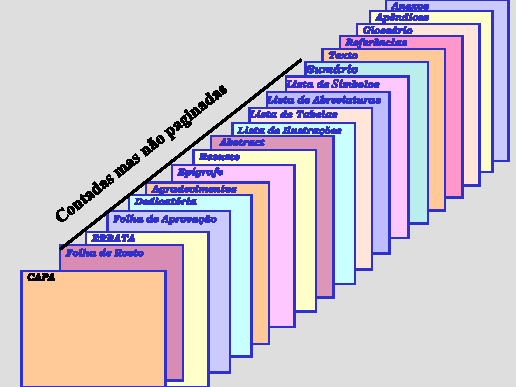
\includegraphics{images/imagem.pdf}
% 	\end{center}
% 	\fonte{Universidade Federal do Paraná (1996).}
% \end{figure}

% % ----------------------------------------------------------
% \subsection{Formatação do texto}
% % ----------------------------------------------------------

% No que diz respeito à estrutura do trabalho, recomenda-se que:
% \begin{alineas}
% 	\item o texto deve ser justificado, digitado em cor preta, podendo utilizar outras cores somente para as ilustrações;
% 	\item utilizar papel branco ou reciclado para impressão;
% 	\item os elementos pré-textuais devem iniciar no anverso da folha, com exceção da ficha catalográfica ou ficha de identificação da obra;
% 	\item os elementos textuais e pós-textuais devem ser digitados no anverso e verso das folhas, quando o trabalho for impresso. As seções primárias devem começar sempre em páginas ímpares, quando o trabalho for impresso. Deixar um espaço entre o título da seção/subseção e o texto e entre o texto e o título da subseção.
% \end{alineas}

% No \autoref{qua:Quadro_1} estão as especificações para a formatação do texto.

% \begin{quadro}[htb]
% 	\centering
% 	\caption{\label{qua:Quadro_1}Formatação do texto.}	
% 	\begin{tabular}{|l|p{11cm}|}
% 		\hline
% 		\textbf{Formato do papel} & A4.\\ \hline
% 		\textbf{Impressão}        & A norma recomenda que caso seja necessário imprimir, deve-se utilizar a frente e o verso da página.\\ \hline
% 		\textbf{Margens}          & Superior: 3, Inferior: 2, Interna: 3 e Externa: 2. Usar margens espelhadas quando o  trabalho for impresso.\\ \hline
% 		\textbf{Paginação}        & As páginas dos elementos pré-textuais devem ser contadas, mas não numeradas. Para trabalhos digitados somente no anverso, a numeração das páginas deve constar no canto superior direito da página, a 2 cm da borda, figurando a partir da primeira folha da  parte textual. Para trabalhos digitados no anverso e no verso, a numeração deve constar no canto superior direito, no anverso, e no canto superior esquerdo no verso.\\ \hline
% 		\textbf{Espaçamento}      & O texto deve ser redigido com espaçamento entre linhas 1,5, excetuando-se as citações de mais de três linhas, notas de rodapé, referências, legendas das ilustrações e das tabelas, natureza (tipo do trabalho, objetivo, nome da instituição a que é submetido e área de concentração), que devem ser digitados em espaço simples, com fonte menor. As referências devem ser separadas entre si por um espaço simples em branco.\\ \hline
% 		\textbf{Paginação}        & A contagem inicia na folha de rosto, mas se insere o número da página na introdução até o final do trabalho.\\ \hline
% 		\textbf{Fontes sugeridas} & Arial ou Times New Roman.\\ \hline
% 		\textbf{Tamanho da fonte} & \textbf{Fonte tamanho 12 para o texto}, incluindo os títulos das seções e subseções. As citações com mais de três linhas, notas de rodapé, paginação, dados internacionais de catalogação, legendas e fontes das ilustrações e das tabelas devem ser de tamanho menor. Adotamos, neste \textit{template} \textbf{fonte tamanho 10}.\\ \hline
% 		\textbf{Nota de rodapé}   & Devem ser digitadas dentro da margem, ficando separadas por um espaço simples por entre as linhas e por filete de 5 cm a partir da margem esquerda. A partir da segunda linha, devem ser alinhadas embaixo da primeira letra da primeira palavra da primeira linha.\\ \hline
% 	\end{tabular}
% 	\fonte{\textcite{NBR14724:2011}.}
% \end{quadro}

% % ----------------------------------------------------------
% \subsubsection{As ilustrações}
% % ----------------------------------------------------------

% Independentemente do tipo de ilustração (quadro, desenho, figura, fotografia, mapa, entre outros), a sua identificação aparece na parte superior, precedida da palavra designativa. 

% \begin{citacao}
% 	Após a ilustração, na parte inferior, indicar a fonte consultada (elemento obrigatório, mesmo que seja produção do próprio autor), legenda, notas e outras informações necessárias à sua compreensão (se houver). A ilustração deve ser citada no texto e inserida o mais próximo possível do texto a que se refere. \cite[p. 11]{NBR14724:2011}.
% \end{citacao}

% % ----------------------------------------------------------
% \subsubsection{Equações e fórmulas}
% % ----------------------------------------------------------

% As equações e fórmulas devem ser destacadas no texto para facilitar a leitura.  Para numerá-las, usar algarismos arábicos entre parênteses e alinhados à direita. Pode-se adotar uma entrelinha maior do que a usada no texto \cite{NBR14724:2011}.

% Exemplos, \autoref{eq:Eq_1} e \autoref{eq:Eq_2}. Observe que o comando \verb|\gls{}| é usado para utilizar para criar um \emph{hyperlink} com a definição do símbolo na lista de símbolos (veja linha 153 de \emph{main.tex}.

% \begin{equation}
% \label{eq:Eq_1}
% \gls{C} = 2 \gls{pi} \gls{r} \sqrt{\gamma} + 10 \, \text{.}
% \end{equation}

% \begin{equation}
% \label{eq:Eq_2}
% \gls{A} = \gls{pi} \gls{r}^2 \, \text{.}
% \end{equation}

% \noindent Aqui não há recuo porque o parágrafo não terminou, apenas foi iniciada uma nova frase após a equação. As equações fazem parte do texto, portanto estão sujeitas à pontuação (ponto final, vírgula etc.).

% % ----------------------------------------------------------
% \subsubsubsection{Exemplo tabela}
% % ----------------------------------------------------------

% De acordo com \textcite{ibge1993}, tabela é uma forma não discursiva de apresentar informações em que os números representam a informação central. Ver \autoref{tab:Tab_1}.

% \begin{table}[htb]
% 	\ABNTEXfontereduzida
% 	\caption{\label{tab:Tab_1}Médias concentrações urbanas 2010-2011.}
% 	\begin{tabular}{@{}p{3.0cm}p{1.5cm}p{2cm}p{2.5cm}p{2.5cm}p{2.5cm}@{}}
% 		\toprule
% 		\textbf{Média concentração urbana} & \multicolumn{2}{l}{\textbf{População}} & \textbf{Produto Interno Bruto – PIB (bilhões R\$)} & \textbf{Número de empresas} & \textbf{Número de unidades locais} \\ \midrule
% 		\textbf{Nome}                      & \textbf{Total}   & \textbf{No Brasil}  &                                                   &                             & \\
% 		Ji-Paraná (RO)                     & 116 610          & 116 610             & 1,686                                             & 2 734                       & 3 082 \\
% 		Parintins (AM)                     & 102 033          & 102 033             & 0,675                                             & 634                         & 683 \\
% 		Boa Vista (RR)                     & 298 215          & 298 215             & 4,823                                             & 4 852                       & 5 187 \\
% 		Bragança (PA)                      & 113 227          & 113 227             & 0,452                                             & 654                         & 686 \\ \bottomrule
% 	\end{tabular}
% 	\fonte{\textcite{ibge2016}.}
% \end{table}
% ---

% ---
% 3 - Capítulo 3
% ---
% ----------------------------------------------------------
\chapter{Project overview}
% ----------------------------------------------------------

% ----------------------------------------------------------
\section{VANT Architecture}
% ----------------------------------------------------------

ProVANT Emergencia is a \gls{UAV} prototype built in 70\% of it's designed size in Belo Horizonte, Brazil\footnotemark, comprised of a fuselage, which houses the electronic components, a V-Tail and wide wings with flaps, ailerons and wingtip nacelles, where the propeller lies. The propellers can rotate 180º to allow for a helicopter like flight and take-off, as can be seen in \autoref{fig:vant}. \cite{merchan_design_2021}

\footnotetext{A 100\% scale version is planned to be build in Universidad de Sevilla}

\begin{figure}[htb]
	\caption{\label{fig:vant}ProVANT Emergencia general mechanical structure view}
	\begin{center}
	    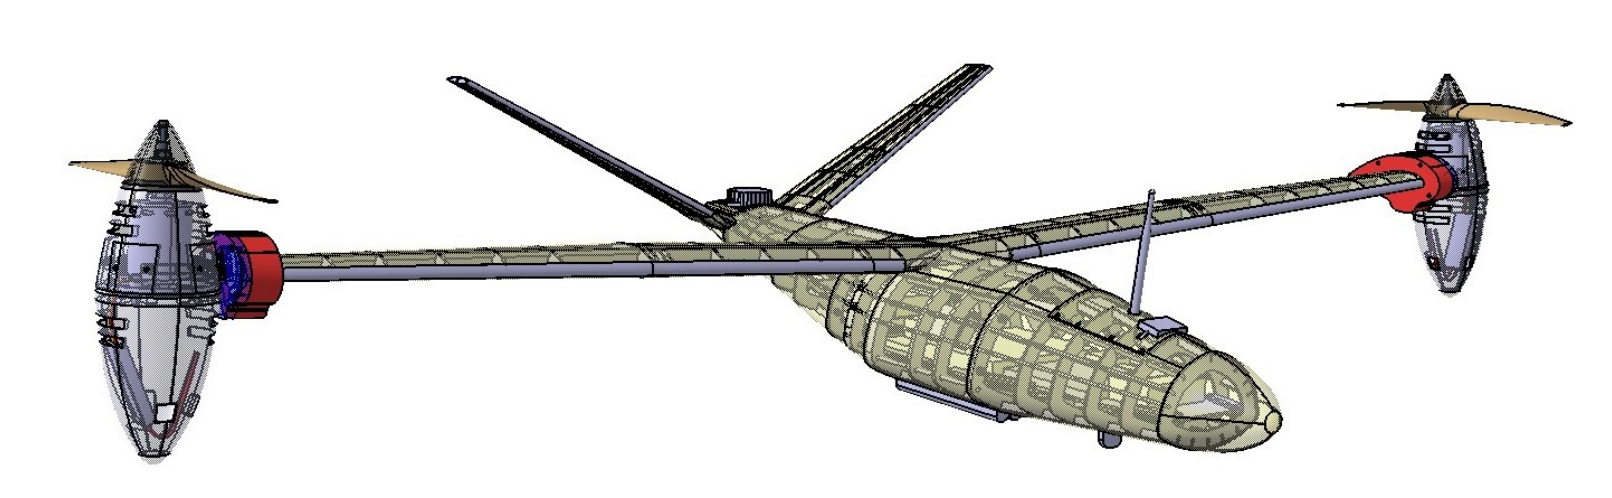
\includegraphics[width=.7\linewidth]{images/VANT.png}
	\end{center}
	\legend{Source: \textcite{merchan_design_2021}.}
\end{figure}

The embedded electronics, as described both by \textcite{lara_design_2019} and \textcite{merchan_design_2021} is developed around two types of embedded processors, called Low Level Hardware (\gls{LLH}) and High Level Hardware (\gls{HLH}). The \gls{LLH} is responsible for directly interfacing with the actuators and simple sensors. It is implemented by two redundant \href{https://www.st.com/en/evaluation-tools/nucleo-f767zi.html}{STM32 Nucleo-F767zi}. 
% Above a referenced the R2U2 site as a citation, here the ST site just by a link, which approach should I used

\begin{figure}[htb]
	\caption{\label{fig:nucleo}ProVANT Emergencia \gls{LLH} board (Nucleo-F767zi)}
	\begin{center}
	    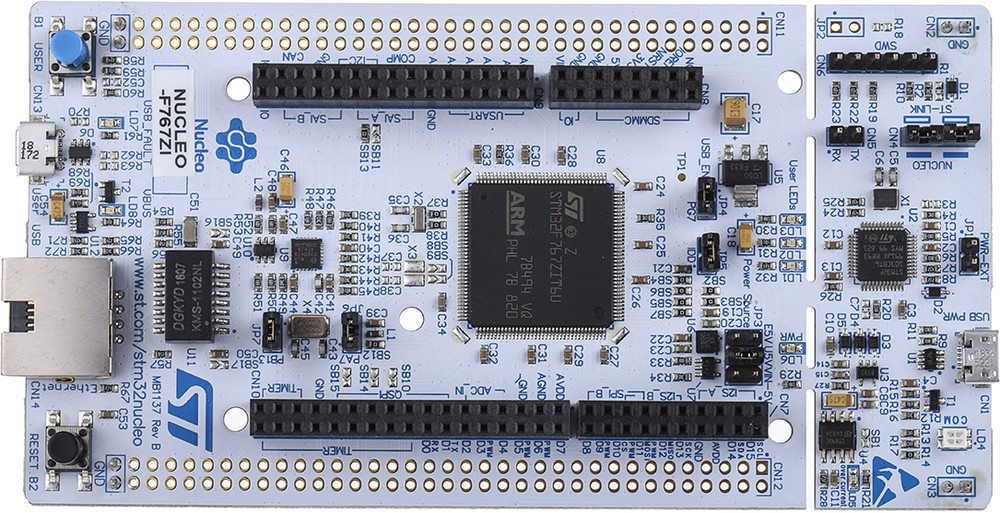
\includegraphics[width=.7\linewidth]{images/nucleo-f767zi.jpg}
	\end{center}
	\legend{Source: From an %russian marketplace 
    advertisement in \href{https://www.chipdip.ru/product/nucleo-f767zi-2}{Chipdip}} % Not great references, but ST website has only low quality images of the board
\end{figure}

The importance of having redundancy in these boards is that they are the only boards in the system with access to the actuators, therefore, in case of a failure in them the system would be incapable of controlling it self.
% if only one board ware used. 
With two Low Level boards, the chances of both failing is much smaller.
% both need to fail to make the system lose access to the actuators, which is a less likely scenario. % more unlikely scenario.

The main \gls{HLH} ti the Jetson Tx2 board, aimed to run the main control loop and chosen by the capability of running neural network, because of it's \gls{GPU} that allows for parallelization of the computing operations. It also interfaces with precise sensors with low latency reading requirements, like the IMU and GPS. \cite{lara_design_2019,merchan_design_2021}

\begin{figure}[htb]
	\caption{\label{fig:jetson}ProVANT Emergencia main \gls{HLH} board (Jetson Tx2)}
	\begin{center}
	    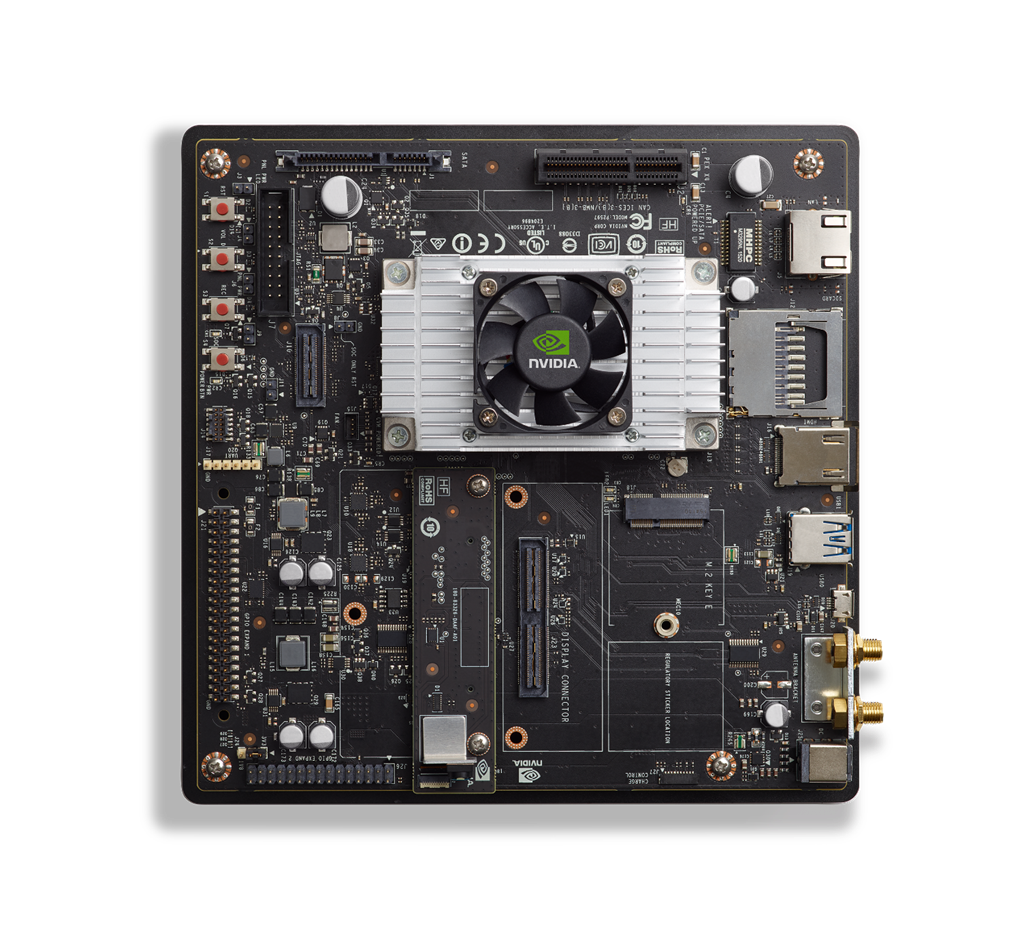
\includegraphics[width=.7\linewidth,trim=2.5cm 2cm 2.5cm 2cm]{images/JTX2_Devkit.png}
	\end{center}
	\legend{Source: From \href{https://www.google.com/url?sa=i\&url=https\%3A\%2F\%2Fdeveloper.nvidia.com\%2Fblog\%2Fjetson-tx2-delivers-twice-intelligence-edge\%2F&psig=AOvVaw1CFt5TyMwmZPdZhERPTBZo\&ust=1727813766519000\&source=images\&cd=vfe\&opi=89978449\&ved=0CBQQjRxqFwoTCMic8oG-64gDFQAAAAAdAAAAABAJ}{Nvidia's website}} 
\end{figure}

Since both aforementioned thesis, a new board was added along the Jetson in the High Level system to interface with the Navio 2 board and a telemetry radio. This board is a Raspberry Pi 4, it facilitates the communication with the Navio 2 board, which implements multiple useful sensors for drones and can generate \gls{PWM} for controlling of actuators. Navio 2 is made to be used with a Raspberry Pi, so using it was the easiest solution.

\begin{figure}[htb]
	\caption{\label{fig:raspberry}ProVANT Emergencia \gls{HLH} auxiliary board (Raspberry Pi 4)}
	\begin{center}
	    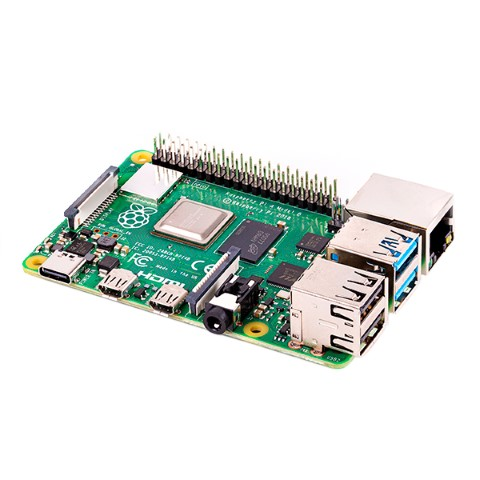
\includegraphics[width=.7\linewidth,trim=.8cm 4cm .8cm 4.3cm,clip]{images/raspberry.png}
	\end{center}
	\legend{Source: From \href{https://www.raspberrypi.com/products/raspberry-pi-4-model-b/}{Raspberry Pi's website}}
\end{figure}

Both Nucleos, the Jetson and Raspberry Pi are connected together in a communication network that implements standards internet protocols, with \gls{UDP} transport layer protocol instead of \gls{TCP}, for it's performance; and Ethernet as physical and link layer protocols. To avoid the non-deterministic characteristics of the standard \gls{CSMA/CD} medium access control protocol, a token ring protocol\footnotemark\ is implemented to avoid collisions.%\cite{noauthor_software_2024} % Não sei se eu posso citar, acho que nunca foi, e talvez nunca será publicado

\footnotetext{This means that only one of the machines will have the permission to use the network hardware. It's said that this board has the "token", and once the permission is given to other board, that the "token was handed" to the other computer.}

\begin{figure}[htb]
	\caption{\label{fig:elecHard}ProVANT Emergencia general electrical structure view}
	\begin{center}
	    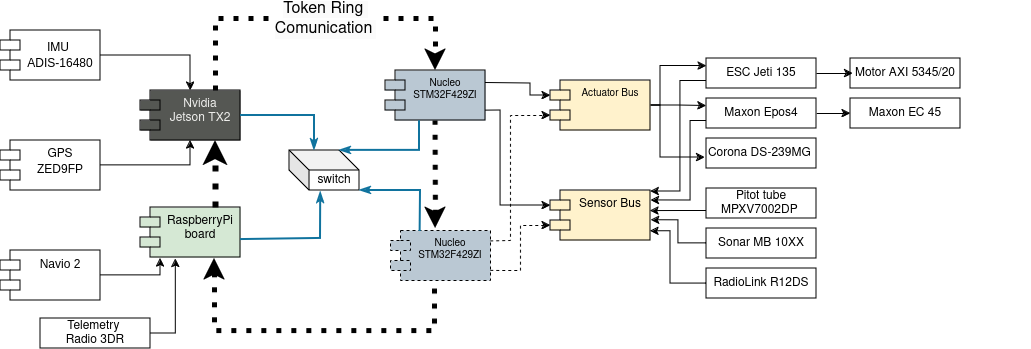
\includegraphics[width=\linewidth,trim=0cm 0cm 2.5cm 0cm,clip]{images/Hardware Setup.png}
	\end{center}
	\legend{Source: 
        %\textcite{noauthor_software_2024}}
        Personal archive} % É do projeto, acho que eu posso por como "pessoal"
\end{figure}


% ----------------------------------------------------------
\section{Fault models for ProVANT}
% ----------------------------------------------------------

When started up, Jetson controls the \gls{UAV} and the primary Nucleo controls the actuators according to the data received from the Jetson. The primary Nucleo should take control if the Jetson enters into a faulty state, likewise the secondary Nucleo has to get the control if both the Jetson and the primary Nucleo fails.

The state of liveliness of each board could be modeled as the \autoref{fig:liveliness}. The composition of this automata for each of the modules is equivalent of the state diagram proposed by \textcite{benica_design_2024} and shown in \autoref{fig:liveliness_full}, where colors are assigned to represent the severeness of the situation.

\begin{figure}[!htb]
    \centering
    \caption{\label{fig:liveliness} Per module liveliness status automata}
    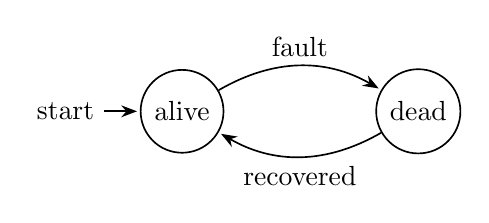
\begin{tikzpicture}[->, >=Stealth, shorten >=1pt, auto, node distance=3cm, semithick]

  \node[state, initial] (q1) {alive};
  \node[state] (q2) [right of=q1] {dead};

  \path (q1) %edge [loop above] node {a} (q1)
            edge [bend left] node {fault} (q2)
        (q2) %edge [loop above] node {c} (q2)
            edge [bend left] node {recovered} (q1);

\end{tikzpicture}
    \legend{Source: Own elaboration}
\end{figure}

\begin{figure}[!htb]
    \centering
    \caption{\label{fig:liveliness_full} Full system liveliness status automata}
    \includegraphics[width=\linewidth,trim=3.2cm 17cm 2.7cm 3cm,clip]{images/Monografia___Daniel_Benicá_liveliness_estate_machine.pdf}
    \legend{Source: \textcite{benica_design_2024}}
\end{figure}

These status should be monitored by each of the modules in order to verify the safeties requirements
and for the correct operation of the token ring protocol, as the tokens shouldn't be given to an unresponsive board. % Need to verify how the token gets transmitted
A possible implementation could be adding a flag at the Module class, or \textit{struct} in case of the c code used in the Nucleos.

To do so, it is necessary to implement techniques to identify faulty boards in the system. As boards should continuously monitor their own behavior with \gls{RV}, it could be the case that a faulty board inform the others about it's faults prior to trying to recover, for example by a reset. However this scenario cannot be considered always possible, unforeseen faults may cause the board to reset or shutdown without warning, or even be unable to communicate.

\textcite{benica_design_2024} proposes methods to identify faults in the system. These methods being: heartbeat, watchdog, network monitoring and exception notification. Heartbeat means periodic messages, called heartbeats, sent by each of the boards inform the normal behavior, missing heartbeats inform a disconnection, this can help to identify a fault on a board that couldn't have communicated it. The watchdog is a timer that needs to be periodically reset by code, allowing the watchdog to overflow could mean the code is not executing or is in a deadlock. Network monitoring is simply calculating the latency of the network and the occurrence of missing messages. Exceptions notification is the common implementation of exceptions in code which can be catch by a catch statement and dealt with in code, one of the proposed ways of dealing with exception was the communication through the network.

\textcite{benica_design_2024} also proposes that the state of each of the boards should follow the \autoref{fig:banica_state}, where the 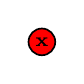
\begin{tikzpicture}[auto, semithick]
\node[draw=black, fill=red, circle, inner sep=0.5mm] {\scriptsize\textcolor{black}{\textbf{x}}};
\end{tikzpicture} symbol represents the possibility of occurring a fault in that state, which triggers a transition to the state marked with 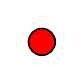
\begin{tikzpicture}[auto, semithick]
\node[draw=black, fill=red, circle, inner sep=0.5mm] {\scriptsize\textcolor{red}{\textbf{x}}};
\end{tikzpicture}.

\begin{figure}[!htb]
    \centering
    \caption{\label{fig:banica_state} State machine for each board}
    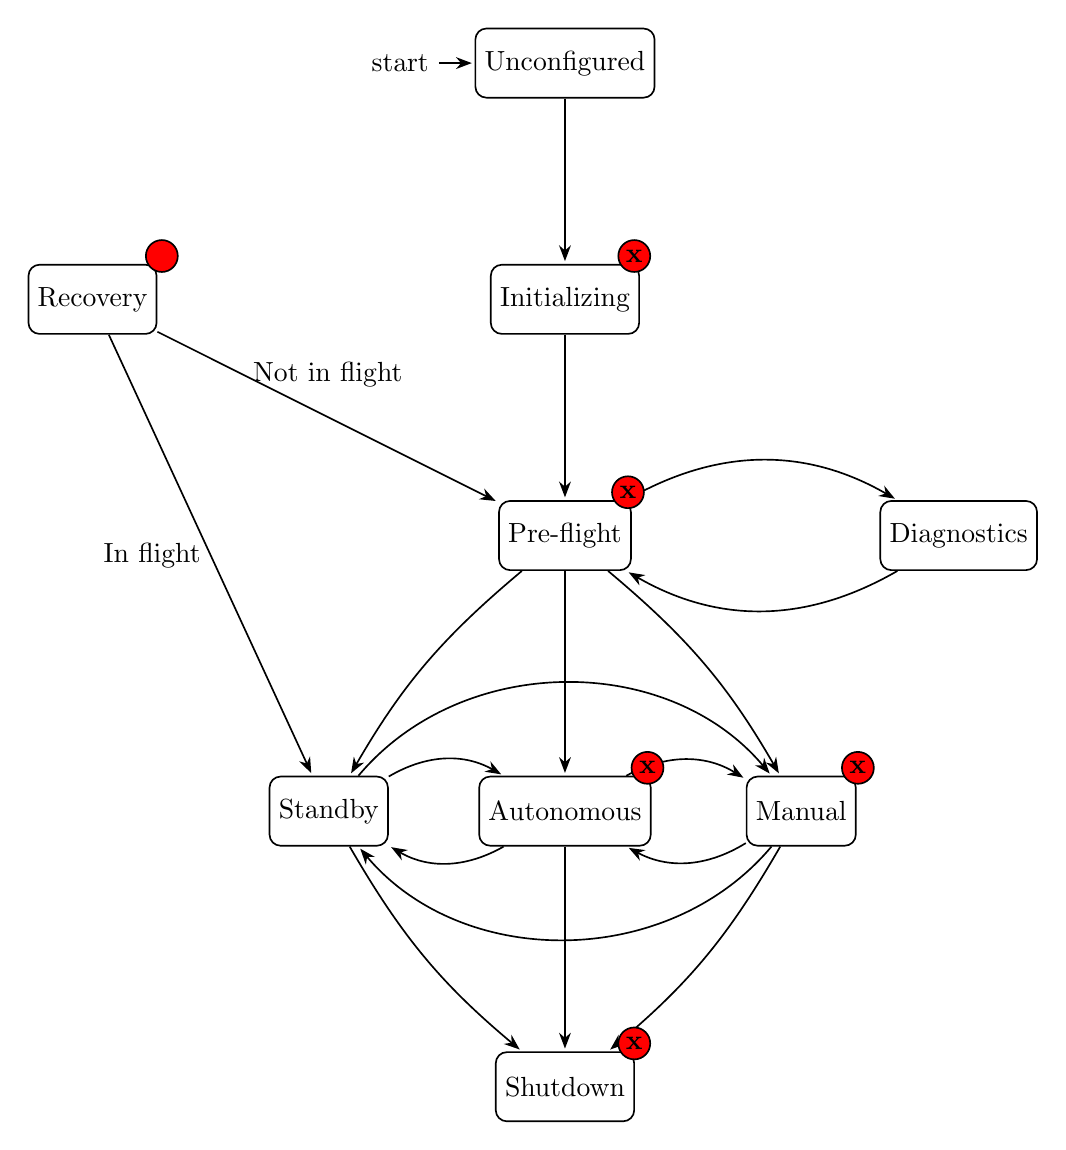
\begin{tikzpicture}[->, >=Stealth, shorten >=1pt, auto, node distance=3cm, semithick]

    % \node[state, initial] (q1) {Unconfigured};
    % \node[state] (init) [below of=q1] {Initializing};
    % \node[state] (pre) [below of=init] {Pre-flight};
    % \node[state] (auto) [below of=pre, yshift=-.5cm] {Autonomous};
    % \node[state] (standby) [left of=auto] {Standby};
    % \node[state] (man) [right of=auto] {Manual};
    % \node[state] (shut) [below of=auto, yshift=-.5cm] {Shutdown};
    % \node[state] (diag) [right of=pre, xshift=2cm] {Diagnostics};
    % \node[state] (recov) [left of=init, xshift=-3cm] {Recovery};

    \node[state, initial, rectangle, rounded corners] (q1) {Unconfigured};
    \node[state, rectangle, rounded corners] (init) [below of=q1] {Initializing};
    \node[state, rectangle, rounded corners] (pre) [below of=init] {Pre-flight};
    \node[state, rectangle, rounded corners] (auto) [below of=pre, yshift=-.5cm] {Autonomous};
    \node[state, rectangle, rounded corners] (standby) [left of=auto] {Standby};
    \node[state, rectangle, rounded corners] (man) [right of=auto] {Manual};
    \node[state, rectangle, rounded corners] (shut) [below of=auto, yshift=-.5cm] {Shutdown};
    \node[state, rectangle, rounded corners] (diag) [right of=pre, xshift=2cm] {Diagnostics};
    \node[state, rectangle, rounded corners] (recov) [left of=init, xshift=-3cm] {Recovery};

  \path (q1) %edge [loop above] node {a} (q1)
            edge node {} (init)
        (init) %edge [loop above] node {c} (q2)
            edge node {} (pre)
        (pre)
            edge [bend right=10] node {} (standby)
        (pre)
            edge node {} (auto)
        (pre)
            edge [bend left=10] node {} (man)
        (standby)
            edge [bend left] node {} (auto)
        (auto)
            edge [bend left] node {} (standby)
        (man)
            edge [bend left] node {} (auto)
        (auto)
            edge [bend left] node {} (man)
        (standby)
            edge [bend left=50] node {} (man)
        (man)
            edge [bend left=50] node {} (standby)
        (auto)
            edge node {} (shut)
        (standby)
            edge [bend right=10] node {} (shut)
        (man)
            edge [bend left=10] node {} (shut);

        \path (pre)
            edge [bend left] node {} (diag)
        (diag)
            edge [bend left] node {} (pre);

        \path (recov)
            edge node [above, yshift=.25cm]{Not in flight} (pre)
        (recov)
            edge node [left]{In flight} (standby);
    
    % \node[draw=black, fill=red, circle, inner sep=0.5mm] at ([xshift=0.88cm, yshift=0.55cm]init) {\textcolor{black}{\textbf{x}}};
    % \node[draw=black, fill=red, circle, inner sep=0.5mm] at ([xshift=0.8cm, yshift=0.5cm]pre) {\textcolor{black}{\textbf{x}}};
    % \node[draw=black, fill=red, circle, inner sep=0.5mm] at ([xshift=1.04797cm, yshift=0.757cm]auto) {\textcolor{black}{\textbf{x}}};
    % \node[draw=black, fill=red, circle, inner sep=0.5mm] at ([xshift=0.72cm, yshift=0.45cm]man) {\textcolor{black}{\textbf{x}}};
    % \node[draw=black, fill=red, circle, inner sep=0.5mm] at ([xshift=0.88cm, yshift=0.55cm]shut) {\textcolor{black}{\textbf{x}}};
    % \node[draw=black, fill=red, circle, inner sep=0.5mm] at ([xshift=0.88cm, yshift=0.55cm]recov) {\textcolor{red}{\textbf{x}}};

    \node[draw=black, fill=red, circle, inner sep=0.5mm] at ([xshift=0.88cm, yshift=0.55cm]init) {\textcolor{black}{\textbf{x}}};
    \node[draw=black, fill=red, circle, inner sep=0.5mm] at ([xshift=0.8cm, yshift=0.55cm]pre) {\textcolor{black}{\textbf{x}}};
    \node[draw=black, fill=red, circle, inner sep=0.5mm] at ([xshift=1.04797cm, yshift=0.55cm]auto) {\textcolor{black}{\textbf{x}}};
    \node[draw=black, fill=red, circle, inner sep=0.5mm] at ([xshift=0.72cm, yshift=0.55cm]man) {\textcolor{black}{\textbf{x}}};
    \node[draw=black, fill=red, circle, inner sep=0.5mm] at ([xshift=0.88cm, yshift=0.55cm]shut) {\textcolor{black}{\textbf{x}}};
    \node[draw=black, fill=red, circle, inner sep=0.5mm] at ([xshift=0.88cm, yshift=0.55cm]recov) {\textcolor{red}{\textbf{x}}};
\end{tikzpicture}
    \legend{Source: \textcite{benica_design_2024} (revised)}
\end{figure}

Problems may arise while integrating the heartbeat technique 
% described by \textcite{benica_design_2024} 
with the token ring protocol, as the designer has decide weither the heartbeat messages should ignore the token, and only data messages have to be send when the board possesses the token, or it should respect the protocol.


% \textbf{Instruções da Coordenação do PFC:}

% Neste capítulo, deve-se apresentar (de forma mais detalhada e aprofundada tecnicamente que na Introdução):
% \begin{itemize}
% 	\item O contexto e a motivação do PFC;
% 	\item Descrição da empresa/instituto de pesquisa (histórico, clientes, produtos, serviços, projetos, etc) em que o PFC foi realizado e do projeto global da empresa em que o PFC está inserido (se for o caso);
%      \item Descrição do problema tratado no PFC;
%      \item Requisitos técnicos (funcionais e não-funcionais).
% \end{itemize}

% Procure utilizar equações, tabelas, diagramas e fluxogramas para ilustrar e explicar melhor as ideias.

% ---

% ---
% 4 - Capítulo 4
% ---
% ----------------------------------------------------------
\chapter{Proposed Method}
% ----------------------------------------------------------

% \textbf{Instruções da Coordenação do PFC:}

% Neste capítulo, deve-se apresentar:
% \begin{itemize}
% 	\item A solução proposta para o problema descrito no capítulo anterior;
% 	\item Explicar a metodologia utilizada na solução proposta;
% 	\item Deixar bem claro e justificar tecnicamente para o leitor como que a solução proposta resolve o problema abordado e atende aos requisitos técnicos, explicando tecnicamente as decisões que foram tomadas para se chegar a tal solução.
% \end{itemize}

% Sugere-se colocar uma diagrama/fluxograma/casos de uso/etc ilustrando a solução proposta, e depois explicar em detalhes cada parte/bloco do diagrama/fluxograma ao longo do texto. 

% Ressaltamos que, em princípio, há uma infinidade de soluções possíveis para o problema abordado no PFC. Desse modo, é preciso explicar detalhadamente e justificar tecnicamente a solução proposta no PFC.

 
% ---

% ---
% 5 - Capítulo 5
% ---
% ----------------------------------------------------------
\chapter{Tests and results}
% ----------------------------------------------------------

% ----------------------------------------------------------
\section{Simulation configuration} 
% ----------------------------------------------------------
O que tava conectado em quê, como pegamos os dados...

% ----------------------------------------------------------
\section{Results}
% ----------------------------------------------------------

% \textbf{Instruções da Coordenação do PFC:}

% Neste capítulo, deve-se:
% \begin{itemize}
% 	\item Descrever detalhadamente como foi feita a implementação/desenvolvimento da solução proposta;
% 	\item Deixar bem claro e justificar tecnicamente para o leitor como que o desenvolvimento realizado implementa de fato a solução proposta, explicando tecnicamente as decisões que foram tomadas para se chegar a tal implentação;
% 	\item Analisar os resultados obtidos com base em indicadores, gráficos, estatísticas, etc: 
% 	\begin{itemize}
% 		\item A implementação realizada solucionou de fato o problema tratado? 
% 		\item Obteve-se o resultado esperado? 
% 		\item Mostrou-se melhor que o método anterior?
% 		\item Vantagens e desvantagens; 
% 		\item Problemas encontrados;   
% 		\item Impacto dos resultados obtidos nos processos/projetos/produtos/serviços/clientes da empresa/instituto de pesquisa; 
% 		\item Impactos organizacionais, tecnológicos, financeiros, éticos, ecológicos, etc.
% 	\end{itemize}
% \end{itemize}

% Sugere-se colocar uma diagrama/fluxograma ilustrando como que a solução proposta foi implementada/desenvolvida, e depois explicar em detalhes cada parte/bloco do diagrama/fluxograma ao longo do texto. 

% Ressaltamos que, em princípio, existe uma infinidade de maneiras diferentes de implementar a solução proposta. Desse modo, o diagrama/fluxograma da solução proposta apresentado no capítulo anterior é mais geral e abstrato que o diagrama/fluxograma da implementação: a implementação realizada no PFC é uma maneira específica de se chegar à solução proposta a partir das técnicas, ferramentas e métodos utilizados. 


% ---

% ---
% 6 - Conclusão
% ---
%\phantompart
% ----------------------------------------------------------
\chapter{Conclusion and future works}
% ----------------------------------------------------------


% \textbf{Instruções da Coordenação do PFC:}

% A Conclusão deve apresentar:
% \begin{itemize}
% 	\item Uma \textbf{síntese} do problema tratado, da solução proposta e dos principais resultados obtidos;
% 	\item Uma discussão sobre o que foi atingido no PFC em relação aos objetivos inicialmente traçados e sobre as limitações encontradas;
% 	\item Uma discussão sobre possíveis aprimoramentos;
% 	\item Destacar os impactos do PFC para a empresa/clientes da empresa/instituto de pesquisa, além de possíveis impactos organizacionais, tecnológicos, financeiros, éticos, ecológicos, etc. 
% 	\item Sugestão de trabalhos futuros (como se poderia dar continuidade ao PFC; aplicar o desenvolvimento realizado no PFC a outros problemas/processos; etc)
% \end{itemize}
% \include{chapters/7-chapter}
% 

\textbf{Instruções da Coordenação do PFC:}

A Conclusão deve apresentar:
\begin{itemize}
	\item Uma \textbf{síntese} do problema tratado, da solução proposta e dos principais resultados obtidos;
	\item Uma discussão sobre o que foi atingido no PFC em relação aos objetivos inicialmente traçados e sobre as limitações encontradas;
	\item Uma discussão sobre possíveis aprimoramentos;
	\item Destacar os impactos do PFC para a empresa/clientes da empresa/instituto de pesquisa, além de possíveis impactos organizacionais, tecnológicos, financeiros, éticos, ecológicos, etc. 
	\item Sugestão de trabalhos futuros (como se poderia dar continuidade ao PFC; aplicar o desenvolvimento realizado no PFC a outros problemas/processos; etc)
\end{itemize}



% ----------------------------------------------------------
% ELEMENTOS PÓS-TEXTUAIS
% ----------------------------------------------------------
\postextual
% ----------------------------------------------------------

% ----------------------------------------------------------
% Referências bibliográficas
% ----------------------------------------------------------
\begingroup
    %\printbibliography[title=REFERÊNCIAS]
    \printbibliography
\endgroup

% ----------------------------------------------------------
% Glossário
% ----------------------------------------------------------
%
% Consulte o manual da classe abntex2 para orientações sobre o glossário.
%
%\glossary

% ----------------------------------------------------------
% Apêndices
% ----------------------------------------------------------

% ---
% Inicia os apêndices
% ---
\begin{apendicesenv}
%	\partapendices* 
	% ----------------------------------------------------------
\chapter{Descrição 1}
% ----------------------------------------------------------

Textos elaborados pelo autor, a fim de completar a sua argumentação. Deve ser precedido da palavra APÊNDICE, identificada por letras maiúsculas consecutivas, travessão e pelo respectivo título. Utilizam-se letras maiúsculas dobradas quando esgotadas as letras do alfabeto. 

\end{apendicesenv}
% ---


% ----------------------------------------------------------
% Anexos
% ----------------------------------------------------------

% ---
% Inicia os anexos
% ---
\begin{anexosenv}
%	\partanexos*
	% ----------------------------------------------------------
\chapter{Descrição 2}
% ----------------------------------------------------------

São documentos não elaborados pelo autor que servem como fundamentação (mapas, leis, estatutos). Deve ser precedido da palavra ANEXO, identificada por letras maiúsculas consecutivas, travessão e pelo respectivo título. Utilizam-se letras maiúsculas dobradas quando esgotadas as letras do alfabeto. 

\end{anexosenv}

%---------------------------------------------------------------------
% INDICE REMISSIVO
%---------------------------------------------------------------------
%\phantompart
%\printindex
%---------------------------------------------------------------------

\end{document}
